\chapter{Diseño}

El robot Scorbot cuenta con una unidad de control propietaria que permite movimiento por ejes y cartesiano a través de un \textit{teach pendant}. También puede ser conectado a un ordenador mediante puerto serial, para el envía de posiciones y trayectorias predefinidas. Lamentablemente el software de control ha quedado obsoleto, pues solo era compatible con MS-DOS, limitando el uso del dispositivo.

Esta limitaciones abren la puerta para el desarrollo de un hardware y software de control del robot, esta vez de basado en herramientas de código libre y estándares industriales que garanticen una mayor vigencia. Además, hacer que el hardware y software del robot sean compatibles con \textit{frameworks} de robótica, reduce el tiempo y dificultad en tareas de integración y creación de nuevas aplicaciones, mejorando su posibilidad de uso futuro.

\section{Controladores} \label{cap3_controladores}

La función principal de los controladores es el manejo del movimiento de un motor DC. Para realizar esta tarea el controlador debe contar con un microcontrolador, encargado de realizar las tareas de computo y comunicación, y una etapa de potencia, quien transfiere al motor los comandos.

Se consideró que los nuevos controladores fueran capaces de, al menos, tener el mismo desempeño que los originales, de esta forma se establecen una serie de requerimientos:

\begin{itemize}
\item Esquema de control distribuido, cada uno de las articulaciones del robot será controlada de forma independiente por un un controlador.
\item Sistema de comunicación capaz de soportar una frecuencia de actualización de 1 \si{\kilo\hertz}.
\item Microcontrolador capaz de establecer un control de corriente a una frecuencia de 10 \si{\kilo\hertz}.
\item La etapa de potencia debe ser capaz de controlar motores DC de 12 \si{\volt} con un consumo \textit{peak} de 8 \si{\ampere}. La frecuencia de conmutación debe ser al menos de 20 \si{\kilo\hertz}, para reducir el rizado de corriente y quede fuera del rango audible. 
\end{itemize}

\subsection{Sistema de comunicación}

Dado que cada articulación del robot esta consitituida por los mismos elementos, parece natural replicar el sistema de control en cada una ellas y establecer sistema de control distribuido. De esta forma, cada una de las articulaciones de controla de forma independiente por un hardware dedicado, denominado esclavo (\textit{slave}). Todos los controladores esclavos son conectados usando un bus de datos con dispositivo maestro (\textit{master}) que establese las referencias de cada controlador.

Uno factor importante en el control distribuido es el tipo de comunicación usado, los pricipales requerimientos para el bus de campo son:
\begin{itemize}
\item Conexión por topología \textit{daisy chain}
\item Protocolo abierto
\item Rápida transmisión de datos y bajo \textit{jitter} 
\item Minimizar el uso de hardware especializado
\end{itemize}

Dados estos creiterios, según \cite{liu2015} el bus de campo EtherCAT el indicado para el diseño de controladores modulares para articulaciones, pues es corresponde a un bus de campo rápido, capaz de alzanr tasas de hasta \SI{100}{Mbit/s} y posee mecanismos de sincronización con una exactitud cercana a los \SI{25}{\nano\second}.

\subsubsection{Uso de librerías de Ethercat}

SOEM
Flanders Mechatronics Technology Centre has decided to release their EtherCAT PR2
Ig gmbh

\subsection{Microcontrolador}

La familia de microcontroladores XMC4 de Infineon Technologies AG esta especilizada para tareas de control de motores y comunicación industrial, por lo que integran hardware especifico para realizar esta tareas. De esta forma, el microcontrolador escogido corresponde al XMC4800, microcontrolador con núcleo ARM Cortex M4 con unidad de punto flotante, incorpora una serie de perifericos útiles utiles para el desarrollo de sistema de control, \textit{timers} de alta resolución para generación de PWM, interfaz para lectura de encoders (POSIF) y módulo comunicación EtherCAT integrado. La Figura \ref{cap3_xmc4800_data} muestra los distintos módulos que posee el XMC4800.

\begin{figure}[ht]
  \centering
  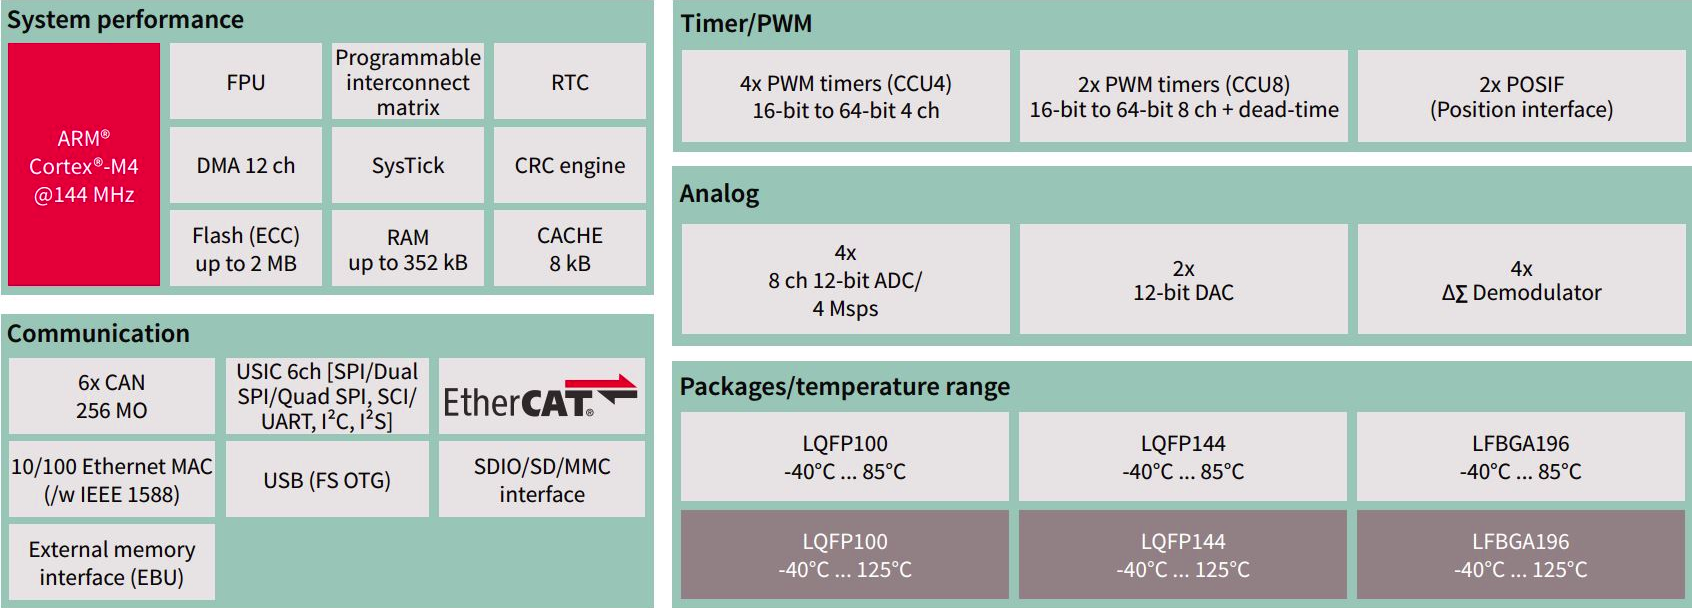
\includegraphics[scale=.2]{img/cap3/xmc4800_data}
  \caption{Carácteristicas del microcontrolador XMC4800. MO: Message Objects, Msps: Mega samples per second.}
  \label{cap3_xmc4800_data}
\end{figure}

La configuración de perifiericos en este tipo de microcontroladores suele ser una tarea compleja, dada las distintos \textit{pin out} y configuraciones de cada uno. Afortunadamente, el fabricante provee un IDE llamado Dave (Digital Application Virtual Engineer) que posee herramientas de generación de código a partir de una interfaz gráfica.

Otra carácteristica importante es que la placa de desarrollo escogida de este microcontrolador, la XMC4800 Relax EtherCAT Kit, posee la mayoría de componentes externos necesarios para el uso de las distintas funcionalidades del microcontrolador, como dos Ethernet PHY (transceiver) para la comunicación EtherCAT. Además integra un programador y debugger Segger J-Link que permite establecer \textit{break points} en el código y acceder a distintos registros de microcontrolador en tiempo real.
 

\subsection{Puente H}

Para la etapa de potencia se selecciono un puente H basado en el IC BTN8982TA, el cual corresponde a un \textit{half bridge} de alta corriente para aplicaciones con motores, contiene 
un MOSFET canal P para el \textit{high-side} y un canal N para el \textit{low-side}, ambos con un driver integrado, que permite su disparo directo desde un microcontrolador.

Para implementación se uso la placa de desarrollo \textit{Motor Control Shield}, que usa dos BTN8982TA en una configuración \textit{full bridge}, las principales carácteristicas:

\begin{itemize}
\item Control bidireccional de motor DC con escobillas de hasta \SI{250}{\watt} continuos.
\item Rango de tensión de entrada nominal \SI{8}{\volt} a \SI{18}{\volt} (\SI{6}{\volt} a \SI{40}{\volt} máximo).
\item Corriente máxima \SI{30}{\ampere}, restringida por la disipación del PCB (BTN8982TA tiene un limite de \SI{55}{\ampere}).
\item Frecuencia de conmutación hasta \SI{30}{\kilo\hertz}.
\end{itemize}




\section{Integración de hardware}

Para reducir el tiempo de desarrollo, se consideró el uso de placas de desarrollo que provee el fabricante. De esta forma se uso kit 

\subsubsection{PCB}

Placa PCB



